\documentclass[twocolumn,aps,prl,amsmath,amssymb,longbibliography]{revtex4-2}
\usepackage{graphicx}
\usepackage{dcolumn}
\usepackage{bm}
\usepackage{amsfonts}
\usepackage{xcolor,tabu}
\usepackage{multirow}
\usepackage{amsthm}
\usepackage{textcomp}
\usepackage{tikz}
\usepackage[colorlinks=true,
            linkcolor=blue,
            urlcolor=blue,
            citecolor=blue]{hyperref}
\hypersetup{bookmarksopen=true}
\usepackage{xr}
% Comment type:
  % -- general comments and communications: questions, uncertainties, marks for further considerations, etc.
  %% -- the original sentence
  %%% -- my changes and reason(s) for the change

% modified sentences will be used in the main text.
% comments will be below the modified sentence

% Things to discuss:
% 1 autocorrelation is included in SI
% 2 alpha=0.5 corresponds to a system with XX. I don't know what XX is supposed to be. Why 0.5?
% 3 I want to avoid the term "cluster", since it sounds more like a "2D" "jammed" state to me.
% 4 Use large graph for energy spectra since there are many curves, put phi dependence as inset
% 5 Confused about units, check Bardfalvy2019
% 6 Particularly, $E(k)$ is flat at small and intermediate $k$ due to the superposition of the dipolar flow fields of uncorrelated bacteria. (don't understand, intermediate k? weak peak?)
% 7 $E(k) = 8\pi/15 n \kappa^2$ (I don't think it's a low k prediction, check Bardfalvy2019)
% 8 Should I indicate the range of fitting in the plot?
% 9 linear plot is also ok for steady-state dN-E plot

\begin{document}

\title{Giant Number Fluctuations and Energy Spectra of 3D Bacterial Suspensions}

\author{Zhengyang Liu}
%\email{liux3141@umn.edu}
\author{Wei Zeng}
\author{Xiaolei Ma}
\author{Xiang Cheng}


\affiliation{Department of Chemical Engineering and Materials Science, University of Minnesota, Minneapolis, MN 55455, USA}

\date{\today}


\begin{abstract}
Giant number fluctuations, a landmark of collectively moving active particles, is universal in active systems across multiple length scales. Here, we present the first experimental study on the giant number fluctuation in 3-dimensional bacterial suspensions. Our measurements show that the number fluctuation scaled by the square root of mean number $\Delta N / \sqrt N$ scales with $N^{0.32}$ at high concentrations, confirming the theoretical predictions. Near the phase boundary, we observe a simultaneous increase of the scaling exponent and the flow induced by bacterial motions, suggesting a strong interplay between giant number fluctuations and flow. We show that this interplay spans all length scales in an active turbulence, by analyzing the kinetic energy spectra.

\end{abstract}

\maketitle

Active fluids exhibit many unusual behaviors beyond the expectation of equilibrium thermodynamics \cite{Ramaswamy2010,Cates2012,Marchetti2013,Poon2013,Elgeti2015}.
In particular, an active fluid exhibits strong transient density inhomogeneity, the so-called giant number fluctuations (GNF), where the variance of particle number shows anomalously strong dependence on the mean number, defying the central limit theorem of equilibrium systems \cite{Mishin2015}.
%% In particular, an active fluid can show anomalously strong density fluctuations, the so-called giant number fluctuations (GNF), where the variance of local particle density is significantly larger than the square root of the mean density, defying the central limit theorem of equilibrium systems \cite{Mishin2015}.
%%% can show anomalously strong density fluctuations --> exhibits strong transient density inhomogeneity
%%%% to avoid repeating "fluctuations"
%%% local particle density is significantly larger than the square root of the mean density --> particle number shows anomalously strong dependence on the mean number
%%%% to variance is std^2 and thus scales with the mean in equilibrium systems // I like to use "number" here in order to be consistent with "giant number fluctuations"
Such anomalous strong number fluctuations have been observed in a wide range of active fluids systems in both living and non-living systems including vibrated granular rods \cite{Narayan2007,Aranson2008,Kudrolli2008,Deseigne2010},
swarming bacteria \cite{Zhang2010,Nishiguchi2017} and mammalian cells \cite{Kawaguchi2017},
self-propelled cytoskeleton \cite{Schaller2013}, and synthetic colloidal swimmers \cite{Palacci2013,Karani2019}. As a result, GNF has generally been viewed as a hallmark of the emergent behaviors of active fluids.
%% Such anomalous density fluctuations have been observed in a wide range of active fluids in both biological and physical systems including vibrated granular rods \cite{Narayan2007,Aranson2008,Deseigne2010}, swarming bacteria \cite{Zhang2010,Nishiguchi2017} and mammalian cells \cite{Kawaguchi2017}, self-propelled cytoskeleton \cite{Schaller2013}, and synthetic colloidal swimmers \cite{Palacci2013,Karani2019}. As a result, GNF has generally been viewed as a hallmark of the emergent behaviors of active fluids.
%%% density --> strong number
%%% biological and physical --> living and non-living
%%%% I feel "physical systems" a little strange but we can talk about this
%%% add ref Kudrolli2008



Significant theoretical and computational advancement on GNF has been made over the past two decades since the seminal works of Toner and Tu \cite{Toner1995,Tu1998,Toner1998,AditiSimha2002,Ramaswamy2003,Toner2005,Chate2008,Mishra2010,
Dey2012,Saintillan2012,Saintillan2013,Ngo2014,Mahault2019}. Meanwhile, many important theoretical and numerical predictions have been tested in experimental realizations
\cite{Narayan2007, Aranson2008, Deseigne2010, Zhang2010, Schaller2013,
Nishiguchi2017, Kawaguchi2017, Palacci2013}.
%% Although significant progress has been made in the theoretical understanding of GNF over the last two decades since the seminal works of Toner and Tu\cite{Toner1995,Tu1998,Toner1998,AditiSimha2002,Ramaswamy2003,Toner2005,Chate2008,Mishra2010, Dey2012,Saintillan2012,Saintillan2013,Ngo2014,Mahault2019}, quantitative experimental verification of many important theoretical and numerical predictions on GNF is still out of reach.
Of particular interest is the scaling exponent $\alpha$, which is defined following $\Delta N /\sqrt N \propto N^\alpha$, where $\Delta N$ is the standard deviation of particle number and $N$ is the mean number of particles in a subsystem of given size. Heretofore, all the existing experiments on GNF were limited to two-dimensional (2D) or quasi-2D systems. In contrast to theoretical predictions (where $\alpha \approx 0.3$), $\alpha$'s obtained in these experiments show large variations ranging from 0.13 to 0.5. Such a large variation arises partially because of complicated particle-boundary interactions, which are hard to incorporate in theoretical studies. Moreover, the predictions of $\alpha$ in three-dimensional (3D) wet active fluids---one of the most important classes of active fluids where hydrodynamics dominate the interparticle interactions and conserve the total momentum of systems \cite{Marchetti2013}---has not been experimentally testified. Therefore, there is an imperative need for an experimental measurement of $\alpha$ in 3D active fluids, which are not affected by system boundaries. Such a measurement will provide not only an unambiguous experimental benchmark to testify theories of active fluids, but also experimental support on the effect of dimensionality on GNF of active fluids \cite{Marchetti2013}.
%% Here, $\alpha$ is defined following $\Delta N /\sqrt N \propto N^\alpha$, where $\Delta N$ is the standard deviation of particle number and $N$ is the mean number of particles in a subsystem of given size.
%% the mean number of particles of a subsystem of given size
%%% of --> in

%% Heretofore, all the existing experiments on GNF were limited to two-dimensional (2D) or quasi-2D systems\cite{Narayan2007, Aranson2008, Deseigne2010, Zhang2010, Schaller2013, Nishiguchi2017, Kawaguchi2017, Palacci2013}. $\alpha$ obtained in 2D experiments shows large variations ranging between 0.13 and 0.5. Such a large variation arises partially because of complicated particle-boundary interactions, which are hard to incorporate in theoretical studies.
%% In contrast, GNF of bulk 3D active fluids are not affected by system boundaries and therefore provides a better control experimental condition for verifying theoretical predictions.

%%% add an before unambiguous
%% Although theoretical prediction of GNF in 2D systems has also been made \cite{Toner1995,Toner2005}, an experimental consensus of the scaling exponent has not been reached.
%%% Rearranged p2 to save space and avoid repetition


The rise of GNF in active fluids is usually accompanied by the transition to ordered phases with collective motions \cite{Ramaswamy2010,Marchetti2013}. For wet 3D active fluids such as bacterial suspensions, these collective motions lead to large-scale coherent flows with intermittent vortices and jets, which are often referred to as active turbulence \cite{Wolgemuth2008,Wensink2012,Dunkel2013a,Bratanov2015,Guo2018,Linkmann2019,Bardfalvy2019,Alert2020,Skultety2020,Peng2020}. Similar to GNF that manifests density fluctuations across different scales, the flow of active turbulence also exhibits scale-dependent structures. Imported from the study of classical turbulence, energy spectra are frequently measured to quantify such structures in active turbulence. Although both GNF and energy spectra quantify the scale-dependent dynamics of active fluids, the deep connection between these two quantities at different scales has not been experimentally investigated. \textcolor{red}{Bridging these two different aspects of active fluids provides new insights into the origin of GNF and reveal hidden dynamic structures of active turbulence.}
% Ths significance statement need further modification

%% frequently measured to quantify such scale-dependent flow properties and to illustrate energy transfer between different scales in active turbulence.
%% Nevertheless, existing experiments on energy spectra of active turbulence all focused on high-concentration suspensions with fully developed active turbulent flows \cite{Ishikawa2011,Wensink2012,Dunkel2013a,Creppy2015,Patteson2018}. How the characteristic turbulent spectrum emerges with increasing particle concentration has not been systematically studied.
%% More importantly, although both GNF and energy spectra quantify the scale-dependent dynamics of active fluids, the intrinsic relation between the two quantities have not been explicitly discussed.

\begin{figure}[ht]
\begin{center}
\includegraphics[width=0.47\textwidth]{Figures/experiment/v1.pdf}
\caption[Experimental details]
{
(a) Bacterial active turbulence displaying constantly varying concentration inhomogeneity (6.4\%). Scale bar is 85 \textmu m.
(b) Velocity field of a dilute bacterial suspension ($\phi=6.4\%$).
(c) Volume fraction as a function of averaged pixel intensities. Inset shows bacterial suspensions of different volume fractions under the same illumination conditions.
(d) Velocity and concentration spatial correlation functions $C_{v}(r)$ and $C_{n}(r)$.
}
\label{fig:experiment}
\end{center}
\end{figure}

In this letter, we present our systematic experimental study of GNF and energy spectra in bulk bacterial suspensions, a premier example of 3D wet active fluids. We use genetically engineered light-powered \textit{Escherichia coli} (\textit{E. coli}) as our model bacteria \cite{Liu2020}.
% \textcolor{red}{Some details about the light-control bacteria and the culturing procedure needed to be given in SM.}
For a typical experiment, a bacterial suspension of control volume fraction $\phi$ is injected into a sealed chamber of $20000 \times 3000 \times 140$ $\mu$m$^3$.
Without supply of oxygen, bacteria quickly consume all the remaining oxygen in the chamber and stop moving after $5$ minutes.
We then illuminate the suspension with light
%% \textcolor{red}{(what type of light? Is the light the same as the microscopy illumination light? Do we saturate the light response of bacteria?The last question is relevant to the next comment below)}
of fixed intensity, which maintains an average swimming speed of bacteria at $11 \pm 1$ $\mu$m/s in the dilute limit.
A video of the active turbulence is then taken 50 $\mu$m above the bottom wall of the chamber by a bright-field inverted microscope at a frame rate of $30$ fps and the field of view of $422 \times 356$ $\mu$m$^2$ (Fig.~\ref{fig:experiment}a).
We use a standard particle image velocimetry (PIV) to extract the 2D in-plane velocity field $(V_x,V_y)$ in the 3D suspension, which exhibits the characteristic collectively-moving vortices and jets of active turbulence at high $\phi$ (Fig.~\ref{fig:experiment}b).

It is challenging to directly count the number of bacteria in a suspension of fasting moving bacteria. Fortunately, the local bacterial density is correlated with the local intensity of microscope images, where darker regions correspond to higher bacterial densities (Fig.~\ref{fig:experiment}a and Supplementary Video). Such a correlation is derived from Beer-Lambert law, the widely used principle of spectrophotometry \cite{Tortora2018}, and has been exploited previously in probing the dynamics in suspensions of bacteria and actin filaments \cite{Sokolov2009, Wilson2011, Schaller2013}.
%Such a correlation derived from the Beer-Lambert law forms the basis of spectrophotometry routinely used in microbiology in measuring bacterial density \cite{Tortora2018} and has also been exploited previously in probing the dynamics in suspensions of bacteria and actin filaments \cite{Sokolov2009, Wilson2011, Schaller2013}.
%Note that the length scale of dense dark clusters is much smaller than the height of the chamber.
% On the macroscopic scale of the chamber, the light intensity is still uniform. \textcolor{red}{This is argument is wrong if the microscopy light is the same as the light power light.} Moreover, the life time of the dense clusters is significantly shorter than the response time of bacteria to the change of light condition. Hence, the motility of light-powered bacteria should not be affected by the local fast light attenuation and is dominantly controlled by the average intensity of illuminating light. \textcolor{red}{We need to justify the formation of clusters does not strongly affect bacteria motility, since in the clusters the light is dimmer. The other argument could be we already saturate the light response of bacteria. Even though in the clusters light is dimmer, bacterial motility is still the same.}
To calibrate the density-intensity correlation, we prepare bacterial suspensions of different volume fractions and image the suspensions under the same illumination (Fig.~\ref{fig:experiment}c inset). The mean image intensity decreases with increasing $\phi$ following an approximately linear relation (Fig.~\ref{fig:experiment}c), agreeing with the the Beer-Lambert law for samples of small thickness and weak absorptivity appropriate for our experiments.

%% \textcolor{red}{I am not sure if this argument is correct. Is there another work showing linear relation too? I remember you mentioned Wilson Poon also found the same linear relation. If yes, we should cite their work here to support our calibration.}
%%% I do have cited (Wilson2011)
%%%%%%%%%%%%%%%%%%%%%%%%%%%%%%%%%%%%%%%%%%%%%%%%%%%%%%%%%%%%%%%%%%%%%%%%%%%%%%%%%%%%%%%%%%
% The argument is correct. In the low attenuation limit (small thickness and weak absorptivity), $I=I_0-\epsilon$ where $\epsilon<<I_0$:
% $$
% \log \frac{I_0}{I} = \log \frac{I_0}{I_0 - \epsilon} \approx \frac{\epsilon}{I_0} \sim c
% $$
% $$
% I = I_0 - \epsilon \sim c
% $$
%%%%%%%%%%%%%%%%%%%%%%%%%%%%%%%%%%%%%%%%%%%%%%%%%%%%%%%%%%%%%%%%%%%%%%%%%%%%%%%%%%%%%%%%%%%

\begin{figure}[ht]
\begin{center}
\includegraphics[width=0.47\textwidth]{figures/GNF/v1.pdf}
\caption[Concentration dependence of GNF.]
{
\textbf{Concentration dependence of GNF.}
(a) Standard deviation of particle number $\Delta N$ scaled by particle mean number $N$ plotted against subsystem size rescaled by single bacterium size $l^2/l_b^2$ in bacterial suspensions at volume fractions ranging from 0.8\% to 9.6\%. Shaded region indicates the range over which the scaling exponents $\alpha$ are fitted.
(b) Concentration dependence of the scaling exponents $\alpha$. Dashed line indicates the high concentration plateau value of $\alpha$ which equals approximately 0.32.
}
\label{fig:GNF}
\end{center}
\end{figure}


\textit{Density fluctuations.}--The linear intensity-density relation allows us to measure the spatiotemporal evolution of relative local bacterial densities and investigate density fluctuations in 3D bacterial suspensions. We first calculate the two-point density spatial correlation and the density auto-correlation for suspensions of different $\phi$ and compare them with well-studied velocity correlations extracted from PIV \cite{Liu2020}.
%% \textcolor{red}{Should we also show autocorrelation? We could have a separate figure for all the four correlations (density, velocity, spatial and auto). In any case, we need to show the definition of the correlation function(s) in SM, if not here in the main text.}
%%%%%%% Done in SM
The correlation length and correlation time are measured when the corresponding correlation functions decay to $1/e$. Fig.~\ref{fig:experiment}d shows the density correlation lengths at different $\phi$
%% \textcolor{red}{(use a symbol different from $l$ for the correlation length, e.g. $\lambda$, since $l$ is used as the size of subsystem below)}
%%%%%%%%%%%%%%% use \lambda: done
, where dense bacterial clusters with a size of $\sim 5$ bacterial lengths emerge in high-concentration bacterial suspensions of $\phi \gtrsim 4\%$.
Simultaneously, long-range correlations also develop in the velocity-velocity correlation, indicating the strong coupling between density fluctuations and collective turbulent flows. The velocity correlation length is about twice of that of density correlations in fully-developed active turbulence.
%% \textcolor{red}{If we show auto-correlation, we need to discuss the correlation time too. The correlation time could be important to justify the 10 frames used in your analysis below.}
%%%%%%% Discuss: autocorrelation is included in SI,

We further examine GNF by calculating the standard deviation of bacterial number $\Delta N$ and the mean bacterial number $N$ in subsystems of increasing sizes \cite{Liu2020}. $\Delta N / \sqrt N$ as a function of $l^2/l_b^2$ for bacterial suspensions of different $\phi$ is plotted in Fig.~\ref{fig:GNF}a, where $l$ is the side length of square subsystems and $l_b=3$ $\mu$m is the average length of bacterial body. Note that the rescaled subsystem size $l^2/l_b^2$ is linearly proportional to mean particle number $N$ at given $\phi$.
%% \textcolor{red}{It is quite confusing that we talked about relative bacterial density in the previous paragraph and then bacterial number in this paragraph. A short explanation on the relation between density and number will help.}
%%%%%%% I don't think so. Density and number has obvious relation $ N = \rho V $
At low $\phi<3.2\%$ where bacterial suspensions do not show active turbulence, $\Delta N$ scales linearly with $\sqrt N$, resulting in constant $\Delta N / \sqrt N$ independent of subsystem sizes. Above $\phi=3.2\%$, bacterial suspensions transition into active turbulence \cite{Peng2020}, where $\Delta N$ increases faster than $\sqrt N$, exhibiting GNF.

The degree of GNF can be quantified by the scaling exponent $\alpha$ from $\Delta N/\sqrt{N} \sim N^\alpha$. $\alpha=0$ for equilibrium systems following the central limit theory, whereas the upper bound $\alpha = 0.5$ corresponds to a system with XX
%% \textcolor{red}{(why 0.5 is maximum?)}.
%%%%%%% Discuss. I don't know what XX is supposed to be.
When the size of subsystems is much larger than the density correlation length $\lambda \approx 5l_b$, the giant fluctuation diminishes due to the averaging over quasi-periodic density patterns (Fig.~\ref{fig:GNF}a) \cite{Saintillan2012}.
%% Note that when the size of subsystems is much larger than the density correlation length $\lambda \approx 5l_b$, the density fluctuation diminishes due to the average of multiple bacterial clusters (Fig.~\ref{fig:GNF}a).
%%%%%%% Discuss: I want to avoid the term "cluster", since it sounds more like a "2D" "jammed" state to me.
Hence, to extract $\alpha$, we fit the experimental curves with power-law relations only in the short length limit (10 to 36 $\mu$m). Fig.~\ref{fig:GNF}b shows $\alpha$ as a function of $\phi$. $\alpha$ remains small at low $\phi$ when the swimming of bacteria is random and increases sharply above $\phi = 3.2\%$ when bacterial suspensions show active turbulence.
$\alpha$ saturates to a high plateau of $0.32 \pm XX$ for $\phi \geq 0.64$, quantitatively agreeing with the theoretical prediction of $\alpha = 1/3$ for 3D suspensions of polar-ordered self-propelled particles with hydrodynamic interactions \cite{AditiSimha2002}. As such, our experiments provide the first quantitative verification of the theoretical prediction on GNF in 3D wet active fluids. Nevertheless, the gradual increase of $\alpha$ at intermediate $\phi$ where active turbulence has already been established cannot been explained by the linear theory. Such a gradual increase has been observed in numerical simulations of suspensions of self-propelled rods beyond the linear regime \cite{Saintillan2012}.

\begin{figure}[!]
\begin{center}\includegraphics[width=0.47\textwidth]{figures/energy-spectra/v1.pdf}
\caption[Concentration dependence of energy spectra.]
{
\textbf{Concentration dependence of energy spectra.}
(a) Energy spectra of bacterial active turbulence at volume fractions ranging from 0.8\% to 9.6\%. Shaded region indicates the range over which the scaling exponents $\beta$ are fitted. Red dashed line is a fitting of the $\phi=0.8\%$ curve (purple), based on the hydrodynamic model of Ref.~\cite{Bardfalvy2019}. Fitting parameters: $n=0.07\%$ and $\epsilon=98$.
(b) Scaling exponents of energy spectra ($\beta$) as a function of volume fractions $\phi$.
}
\label{fig:energy-spectra}
\end{center}
\end{figure}

\textit{Energy spectra.}--
Like GNF, the velocity field of active turbulence also shows scale-dependent structures.
%% While GNF quantifies the density fluctuations of active turbulence at different length scales, the velocity field of active turbulence also shows scale-dependent structures.
%%
We investigate such structures by calculating the energy spectra of bacterial suspensions $E(k)$ at different $\phi$ \cite{Liu2020}. $E(k)$ measures the kinetic energy density at different scales in terms of wavenumber $k = 2\pi/l$, which is related to the real-space mean kinetic energy density $E = \langle V_x^2 + V_y^2 \rangle/2$ via $E = \int_0^\infty E(k)dk$. Fig.~\ref{fig:energy-spectra}a shows $E(k)$ of bacterial suspensions at different $\phi$.
%% \textcolor{red}{We should plot $k/k_b$, instead of $k$ in analogy of $l/l_b$ for GNF.}
%%%%%%%%%%%%% Done
At low $\phi$ with random swimming bacteria, $E(k)$ quantitatively agrees with the theoretical prediction for uncorrelated pusher swimmers \cite{Bardfalvy2019}
\begin{equation}
E_k = 4\pi n \kappa^2 \left[ \frac{1}{3} + \frac{\cos(kl)}{(kl)^2} - \frac{\sin(kl)}{(kl)^3} \right] \frac{\epsilon^4k^2}{l^2} K_2^2(k\epsilon)
\end{equation}
where  $\kappa \approx 11.2$ is the stresslet strength of \textit{E. coli}, $l\approx 1.9$ is the dipolar length, $\epsilon$ is a factor describing the distance over which the regularisation acts and $K_2$ is the modified Bessel function of the second kind. The fitting parameters $n$ and $\epsilon$ are found to be 0.07\% and 98, respectively.
%%\textcolor{red}{Show the fitting equation and explain the meaning of the symbols.}
%%%%%%%%%%%%%% Confused about units, check the paper
Particularly, $E(k)$ is flat at small and intermediate $k$ due to the superposition of the dipolar flow fields of uncorrelated bacteria.
%%%%%%%%%%%%% Discuss: I don't understand
%% \textcolor{red}{The theory shows $E(k) = 8\pi/15 n \kappa^2$ in the low $k$ limit, where $\kappa = Fl/\eta$ with $Fl$ the dipole strength and $\eta$ viscosity. Does this prediction quantitatively agree with our measurements?}
%%%%%%%%%%%%% Discuss: I don't think it's a low k prediction.
%% $E(k)$ at small $k$ increases with $\phi$.
At high $\phi$ in the turbulent regime, although the energy is injected by a single bacterium at small scales, the kinetic energy is concentrated at scales much larger than the size of single bacteria $l_b$.
Weak peaks are observed for high $\phi$ suspensions at low $k$. The trend qualitatively agrees with numerical results \cite{Saintillan2012,Bardfalvy2019}. We also extract the scaling exponent $\beta$ from $E(k) \sim k^{-\beta}$ by fitting the energy spectrum curves at intermediate $k$, where a significant change of $E(k)$ with $\phi$ occurs and $E(k)$ exhibits good power-law relations.
%% \textcolor{red}{I think we should use a smaller range of $k$ in the fitting. For the low $\phi$ samples, the curves are apparently nonlinear in the current range.I don't think we need to enforce the overlap of the length scales between GNF and energy spectra at this point, since we will plot $\Delta N/\sqrt{N}$ and $E(k)$ directly anyway.}
%%%%%%%%%%%%%%% Sure
$\beta$ increases with $\phi$ and saturates at $2.9 \pm 0.1$ at high $\phi$, similar to the trend of $\alpha$. The saturated scaling exponent is consistent with that reported by previous experiments on active turbulence of high-concentration suspensions \cite{Wensink2012,Creppy2015,Patteson2018}, but smaller than the prediction of simulations and theories at 4 in the high $k$ limit
\cite{Saintillan2012,Giomi2015,Bardfalvy2019}. To the best of our knowledge, our study provides the first systematic experimental results on the evolution of $E(k)$ over a large range of $\phi$ of bacterial suspensions.

\begin{figure}[!]
\begin{center}
\includegraphics[width=0.47\textwidth]{figures/GNF-energy-spectra-correlation/v1.pdf}
\caption[The correlation between GNF and kinetic energy and kinetic energy spectra.]
{
\textbf{The correlation between GNF and kinetic energy and kinetic energy spectra.}
(a) Local correlations between density fluctuations and kinetic energy at volume fractions ranging from 0\% to 9.6\%. Inset: a snapshot of a density fluctuation field and a kinetic energy field. The correlations are calculated by averaging over 1000 frames.
(b) Energy spectra $E$ plotted against number fluctuations ($\Delta N/\sqrt N$) at corresponding length scales at volume fractions ranging from 0\% to 9.6\%. Black arrow indicates the direction of increasing length scale. Inset: the scaling exponent of number fluctuations $\alpha$ plotted against the scaling exponent of energy spectra $\beta$ at corresponding volume fractions.
}
\label{fig:GNF-energy-spectra-correlation}
\end{center}
\end{figure}

\textit{Density-flow coupling.}--Both GNF and energy spectra probe the scale dependence of active turbulence. The former measures the density fluctuations at different scales, whereas the latter considers the flow energy across scales. Although both quantities have been extensively studied, the coupling between the two has not been explicitly examined so far. A quantitative understanding of this coupling will reveal the hidden correlation between density fluctuations and flow structures at different scales.
%% First, at large scales, it is apparent that density fluctuations positively correlate the overall kinetic energy.
A high-$\phi$ suspension deep in the turbulent regime exhibits both strong density fluctuations and large kinetic energy (Fig.~\ref{fig:GNF} and \ref{fig:energy-spectra}). To further illustrate the correlation between density fluctuations and the kinetic energy of turbulent flows at microscopic scales, we measure the \emph{local} correlation of the two quantities. Specifically, we divide the images of bacterial suspensions into small square windows of size $17$ $\mu$m. The standard deviation of the density of each window at time $t$, $\delta N(\vec{r},t)$, is then calculated over a small time interval of $0.3$ s, much less than the correlation time of density $\tau$.
%% less than the correlation time of density fluctuations $\tau$.
$\delta N(\vec{r},t)$ quantifies the local density fluctuation at position $\vec{r} = (x,y)$ and time $t$ (Fig.\ref{fig:GNF-energy-spectra-correlation}a inset).
The same windows are then also used in PIV to extract the local velocities of bacterial suspensions. The local kinetic energy at $t$ is given by $E_l(\vec{r},t) = \left[ V_x(\vec{r},t)^2 + V_y(\vec{r},t)^2 \right]/2$ (Fig.\ref{fig:GNF-energy-spectra-correlation}a inset). Finally, the correlation between $\delta N(\vec{r},t)$ and $E_l(\vec{r},t)$ is defined as
\begin{equation}
C = \bigg \langle \frac{ (\delta N(\vec{r},t) - \langle \delta N(\vec{r},t) \rangle_r)(E_l(\vec{r},t) - \langle E_l(\vec{r},t) \rangle_r)}{\sigma_{\delta N}\sigma_{E_1}} \bigg \rangle,
\end{equation}
where $\langle X \rangle_r$ and $\sigma_X$ are the mean and standard deviation of $X$ over the space $\vec{r}$, respectively, and the average $\langle\cdot\rangle$ is taken over all $x$, $y$ and $t$.
%% \textcolor{red}{Fill in the formula here.}
Fig.\ref{fig:GNF-energy-spectra-correlation}a shows $C$ as a function of $\phi$. At low $\phi$ with random swimming bacteria, the correlation between density fluctuations and kinetic energies remains weak fluctuating around zero. The correlation increases with $\phi$ as bacterial suspensions transition to active turbulence. An obvious positive correlation can be observed in the turbulent regime with $\phi \ge 4\%$, consistent with the observation at large scales.

The correlations at both large and small scales imply that density fluctuations and kinetic energies may be correlated across all length scales in active turbulence. A scale-independent correlation between density fluctuations and kinetic energies may exist. Indeed, when we plot density fluctuations $\Delta N/\sqrt N$ against the corresponding kinetic energies $E$ at the same scale, all the $\Delta N/\sqrt N$-$E$ pairs fall onto a universal curve in the active turbulence regime over \textcolor{red}{two (17 $\mu$m PIV box to the field of view length scale)} orders of magnitude in scales, regardless of the specific volume fractions of the samples.
%% \textcolor{red}{I am wondering if we should plot the data in a linear-linear plot, which may show better data collapse. The dynamic range of the collapsing is barely one decade in $y$ and only a factor of 2 in $x$.}
%%%%%%%%%%%%%%%% Discuss: linear plot is also ok
In contrast, $\Delta N/\sqrt N$-$E$ shows much stronger scattering for low $\phi$ suspensions with random swimming bacteria. We also plot $\alpha$ versus $\beta$ to compare the scaling exponents of the two variables. We find $\alpha$ increases linearly with $\beta$ with a constant ratio $\alpha/\beta = 0.087 \pm 0.012$ in the turbulent regime. The result further strengthens the strong scale-independent correlation between the density fluctuations and the kinetic energy of active turbulent flows.

In summary, we present the first measurement on GNF in 3-dimensional bacterial suspensions. The scaling exponents $\alpha$ we measure are not subject to the effect of frictional walls and are thus more suitable for quantitatively testing theoretical predictions.
Our detailed analysis on the velocity fields reveals a strong coupling between flow kinetic energy and GNF, not only on the global scale, but spans all the length scales down to single swimmer length.
Our measurements will contribute to the advancement of quantitative understanding of collective motions and GNF in bacterial active turbulence.

\bibliographystyle{apsrev4-2}
\bibliography{correlation}



\end{document}
